\section{Séance 9}

\subsection{Retourner un graphe planaire}
Donnez une autre représentation planaire du graphe suivant où la face spécifiée (egf) devient la face extérieure.

\begin{figure}[h!]
  \begin{center}
    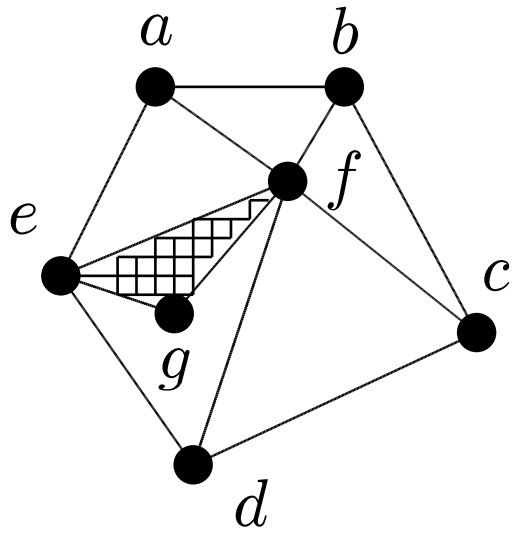
\includegraphics[width=4cm]{tp9_1.png}
      \end{center}
\end{figure}

\begin{solution}
  \begin{center}

    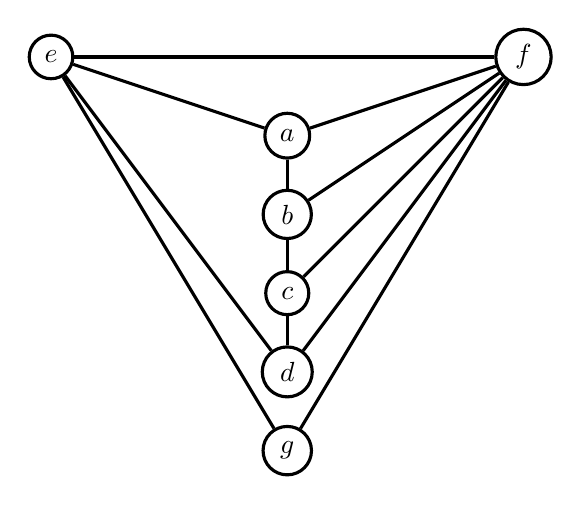
\begin{tikzpicture}[scale=1,looseness=1,auto,line width=.4mm]
      \path (0, -1) node[draw,shape=circle] (1)  {$a$};
      \path (0, -2)  node[draw,shape=circle] (2)  {$b$};
      \path (0,-3) node[draw,shape=circle] (3)  {$c$};
      \path (0, -4) node[draw,shape=circle] (4)  {$d$};
      \path (-3, 0) node[draw,shape=circle] (5)  {$e$};
      \path (3, 0) node[draw,shape=circle] (6)  {$f$};
      \path (0, -5) node[draw,shape=circle] (7)  {$g$};

      \draw (1) -- (2);
      \draw (1) -- (5);
      \draw (1) -- (6);
      \draw (2) -- (3);
      \draw (2) -- (6);
      \draw (3) -- (4);
      \draw (3) -- (6);
      \draw (4) -- (5);
      \draw (4) -- (6);
      \draw (5) -- (6);
      \draw (5) -- (7);
      \draw (6) -- (7);

    \end{tikzpicture}
  \end{center}
\end{solution}


\subsection{Cylindre bi-infini}
Un graphe planaire peut-il être représenté sur un cylindre bi-infini sans ses arêtes ne se croisent? La réciproque est-elle vraie?  Et pour un graphe sur un tore?

\begin{solution}
Pour le cylindre bi-infini : 
\begin{itemize}
\item plan $\longrightarrow$ cylindre : oui, il suffit de découper un carré contenant le graphe et de joindre les 2 côtés opposés
\item cylindre $\longrightarrow$ plan : oui, il suffit de projeter le ``haut'' du cylindre dans un point unique du plan, et le ``bas'' à l'infini. \\
\end{itemize}

Pour le tore : 
\begin{itemize}
\item plan $\longrightarrow$ tore : idem plan $\longrightarrow$ cylindre
\item tore $\longrightarrow$ plan : non, car on peut dessiner le graphe $K_5$ sur un tore sans que ses arêtes ne se croisent (l'une des arêtes fait le tour du tore).
\end{itemize}
\end{solution}

\subsection{Graphes planaires ?} Les graphes suivants sont-ils planaires?

\begin{figure}[h!]
  \begin{center}
    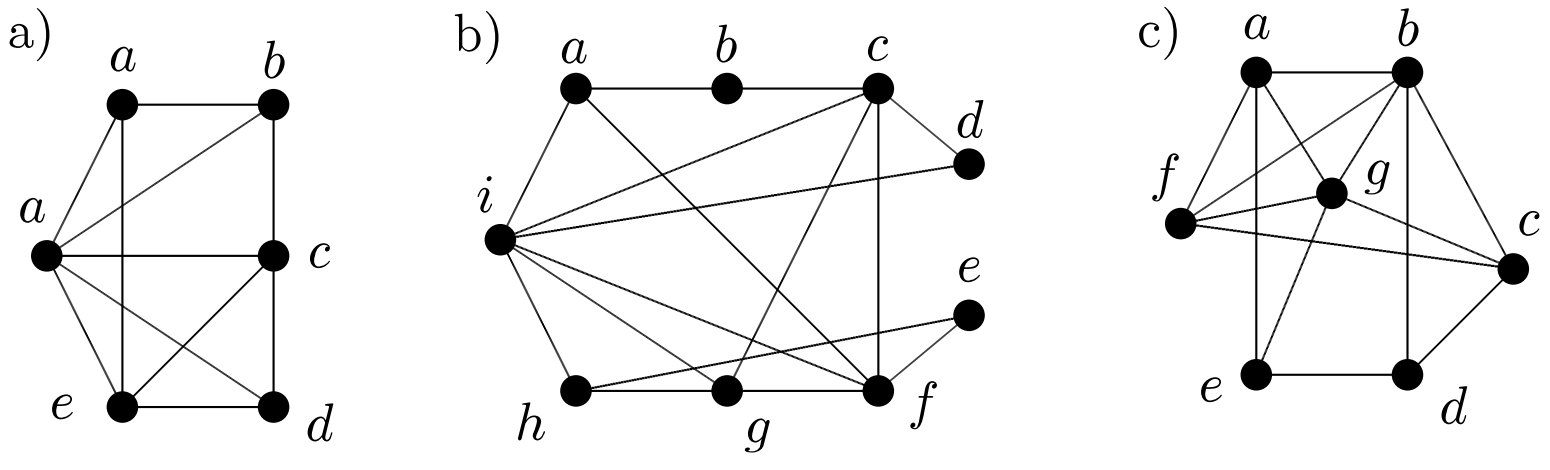
\includegraphics[width=15cm]{tp9_2.png}
      \end{center}
\end{figure}

\begin{solution}
  \begin{center}
    \begin{tabular}{lcr}
      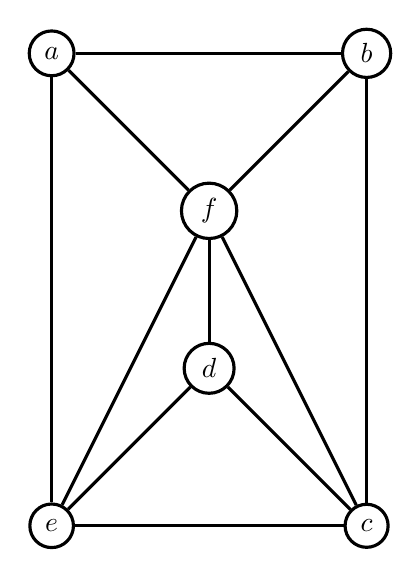
\begin{tikzpicture}[scale=1,looseness=1,auto,line width=.4mm]

        \path (-2,3) node[draw,shape=circle] (1)  {$a$};
        \path (2,3) node[draw,shape=circle] (2)  {$b$};
        \path (2,-3) node[draw,shape=circle] (3)  {$c$};
        \path (0,-1) node[draw,shape=circle] (4)  {$d$};
        \path (-2,-3) node[draw,shape=circle] (5)  {$e$};
        \path (0,1) node[draw,shape=circle] (6)  {$f$};

        \draw (1)  -- (2);
        \draw (1)  -- (5) ;
        \draw (1)  -- (6)  ;
        \draw (2)  -- (3)  ;
        \draw (2)  -- (6)  ;
        \draw (3)  -- (6)  ;
        \draw (3) -- (4) ;
        \draw (3) -- (5) ;
        \draw (4) -- (6) ;
        \draw (4)  -- (5) ;
        \draw (5)  -- (6)  ;
      \end{tikzpicture}

      & \hspace{0.5cm} &
      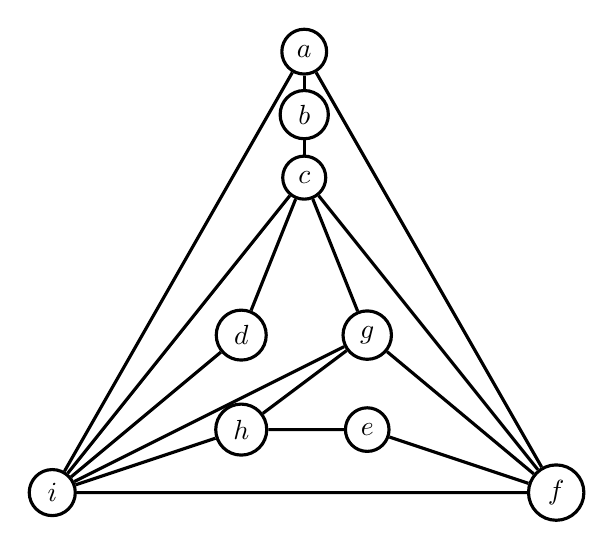
\begin{tikzpicture}[scale=0.4,looseness=1,auto,line width=.4mm]

        \path (0,0) node[draw,shape=circle] (1)  {$a$};
        \path (0,-2) node[draw,shape=circle] (2)  {$b$};
        \path (0,-4) node[draw,shape=circle] (3)  {$c$};
        \path (-2,-9) node[draw,shape=circle] (4)  {$d$};
        \path (2,-12) node[draw,shape=circle] (5)  {$e$};
        \path (8,-14) node[draw,shape=circle] (6)  {$f$};
        \path (2,-9) node[draw,shape=circle] (7)  {$g$};
        \path (-2,-12) node[draw,shape=circle] (8)  {$h$};
        \path (-8,-14) node[draw,shape=circle] (9)  {$i$};

        \draw (1)  -- (2);
        \draw (1)  -- (6);
        \draw (1)  -- (9);
        \draw (2)  -- (3);
        \draw (3)  -- (4);
        \draw (3)  -- (6);
        \draw (3) -- (7) ;
        \draw (3) -- (9) ;
        \draw (4) -- (9) ;
        \draw (5)  -- (6);
        \draw (5)  -- (8);
        \draw (6)  -- (7);
        \draw (6) -- (9) ;
        \draw (7) -- (8) ;
        \draw (7) -- (9) ;
        \draw (8)  -- (9);

      \end{tikzpicture}

    \end{tabular}
  \end{center}

  Le graphe c) n'est pas planaire.
  En effet, on observe que le graphe possède une clique de 4 noeuds $(a,b,g,f)$.
  On observe aussi que le noeud $c$ est adjacent à $b, g$ et $f$.
  On prouve ensuite qu'il existe un chemin entre $c$ et $a$ qui ne passe pas par $b$, $g$ ou $f$:
  le chemin $c-d-e-a$. Cela signifie qu'il existe un sous-graphe $K_5$ ``caché'' dans le graphe. Or,

  \begin{quotation}
    ``Un graphe est non planaire si et seulement s’il contient comme sous-graphe $K_5$ ou $K_{3,3}$ ou une subdivision de ceux-ci.''
  \end{quotation}

\end{solution}

\subsection{Division en face}
Supposez qu’un graphe connexe planaire a 6 sommets, chacun de degré 4. En combien de régions le plan est-il divisé par une représentation planaire de ce graphe?

\begin{solution} Soit $n = 6$, $e = \frac{6 \cdot 4}{2}$. Par la formule d'Euler $ n - e + f = 2$, on a : $f = 2 - 6 + 12 = 8$.
\end{solution}

\subsection{Graphe ou complémentaire non-planaire}
Le complémentaire $\bar{G}$ d’un graphe $G = (V,E)$ de $n$ sommets est donné par $\bar{G} = (V, E(K_n) - E)$. Montrez que si $n \geq 11$, au moins un des deux graphes $G$ ou $\bar{G}$ n’est pas planaire.

\begin{solution} Pour tout graphe planaire simple à $n$ sommets, le nombre d'arêtes $e$ est défini par la borne supérieure  $e \leq 3n - 6$. \\
On sait que $|E(K_{n})| = \frac{n(n-1)}{2} = |E(G)| + |E(\bar{G})|$. \\
Pour qu'à la fois $G$ et $\bar{G}$ soient planaires, il faut que 
\[ \begin{array}{rcl}
 \frac{n(n-1)}{2} &\leq& 2 (3n - 6) \\
  n(n-1) &\leq& 4(3n - 6) \\
  n^2 - 13n + 24 \leq 0 \\
 \end{array} \]
 
 En résolvant l'équation du deuxième degré, on obtient les racines $10.7720$ et $2.2280$, ce qui signifie que pour que les deux graphes $G$ et $\bar{G}$ soient planaires, il faut que $2.2280 \leq n \leq 10.7720$.
 \end{solution}

\subsection{Conservation de la planarité}
Sous quelle condition est-il possible d’ajouter une arête à un graphe planaire en conservant la planarité ? Déduisez le nombre total d’arêtes qu’il est possible d’ajouter à un graphe planaire de $n$ sommets et $m$ arêtes tout en conservant la planarité.

\begin{solution} Le nombre maximal d'arêtes que l'on peut mettre dans un graphe planaire est $e = 3n - 6$ Soit $x$ le nombre d'arêtes que l'on peut ajouter à un graphe de $m$ arêtes tout en conversant la planarité. On a donc $e = m + x$, ce qui donne $x = 3n - 6 - m$. Notons que la formule d'Euler ($ n - e + f = 2$) nous dit que $x$ est aussi le nombre maximum de faces que l'on peut ajouter au graphe planaire de $n$ sommets et $m$ arêtes. 
\end{solution}

\subsection{Nombre de faces}
Soit un graphe $G$ 3-régulier tel que tout sommet est incident à une face de degré 4, une face de degré 6 et une face de degré 8. Sans dessiner $G$, déterminez le nombre de faces de $G$.

\begin{solution} Un noeud ne peut être incident qu'à une seule face de degré 4, une seule face de degré 6 et une seule face de degré 8. Si on désigne
\begin{itemize}
\item $f_4$ le nombre de faces de degré 4,
\item $f_6$ le nombre de faces de degré 6, et
\item $f_8$ le nombre de faces de degré 8;
\end{itemize}
on peut donc dire que $n = 4f_4 = 6f_6 = 8f_8$, et donc : 
\[  
\begin{array}{rcl}
f &=& f_4 + f_6 + f_8 \\
  &=& \frac{n}{4} + \frac{n}{6} + \frac{n}{8} \\
  &=& \frac{6 + 4 + 3}{24} n \\
  &=& \frac{13}{24} n 
\end{array}
\]

Sachant que $e = \frac{3n}{2}$, on a, par la formule d'Euler, $$ n - \frac{3n}{2} + \frac{13}{24} n = 2 $$
On trouve donc que $$ n = 48 \qquad e = 72 \qquad f = 26$$
$$ f_4 = 12 \qquad f_6 = 8 \qquad f_8 = 6$$
\end{solution}

\subsection{Coloriage des faces}
Montrez que si tous les sommets d’un graphe planaire $G$ sont de degré pair, alors toutes les faces de $G$ peuvent être coloriées en deux couleurs de telle sorte que deux faces adjacentes n’aient jamais la même couleur.

\begin{solution}
Si toutes les coupes dans le graphe $G$ comportent un nombre pair d'arêtes, cela signifie que les cycles dans le graphe dual seront de longueurs paires également.
En effet, une coupe dans le graphe $G$ est l'équivalent du cycle enfermant une face dans le graphe dual.
Nous allons montrer que toutes les coupes dans $G$ comportent un nombre pair d'arêtes.

Tous les sommets de $G$ étant de degré pair, il existe un parcours Eulerien fermé dans $G$.
Comme le parcours couvre toutes les arêtes du graphe et retourne à son point de départ, une coupe le traverse toujours un nombre pair de fois: pour toute arête qui passe de l'autre côté de la coupe, il doit en exister une complémentaire qui revient dans l'autre sens pour fermer le parcours.

Ceci implique que tous les cycles du dual de $G$ sont pairs, et donc que le dual de $G$ est biparti.
S'il est biparti, on peut le colorier avec deux couleurs.
\end{solution}

\subsection{Impression de circuits électriques}
Un circuit électrique connecte des terminaux de deux types $A$ et $B$. Chaque terminal $A$ est connecté à chaque terminal $B$. Montrez qu’un tel circuit peut être imprimé sur les deux faces d’une seule feuille isolante si les terminaux traversent la feuille.

\begin{solution}
  \nosolution
\end{solution}
